\section{Izvanmrežni način rada}

Penjališta se često nalaze na udaljenim lokacijama s ograničenim ili nepostojećim internetskim signalom. Zbog toga aplikacija implementira izvanmrežni način rada kako bi omogućila korisnicima korištenje aplikacije i situacijama slabog internetskog signala. Ova mogućnost je dostupna samo na mobilnoj aplikaciji. Korisnik može preuzeti podatke za bilo koje penjalište ili penjački smjer unutar detaljnog pregleda penjališta ili penjačkog smjera klikom na "Preuzmi penjalište" (eng. \textit{Download crag}) ili "Preuzmi penjački smjer" (eng. \textit{Download route}). Aplikacija tada pohranjuje sve podatke na lokalni uređaj, uključujući informacije o sektorima i penjačkim smjerovima, galerije forografija te najvažnije, referentne slike penjačkh smjerova potrebne za rad funkcionalnosti prepoznavanja penjačkih smjerova.

\begin{figure}[H]
    \centering
    \begin{subfigure}[b]{0.4\textwidth}
        \centering
        \includegraphics[width=0.7\textwidth]{images/implementacija/offline-mode/crag-tab.png}
        \caption{Popis preuzetih penjališta}
        \label{fig:offline_crag_tab}
    \end{subfigure}
    \hspace{0.08\textwidth}
    \begin{subfigure}[b]{0.4\textwidth}
        \centering
        \includegraphics[width=0.7\textwidth]{images/implementacija/offline-mode/routes-tab.png}
        \caption{Popis preuzetih penjačkih smjerova}
        \label{fig:offline_routes_tab}
    \end{subfigure}
    \caption{Izvanmrežni način rada - pregled preuzetih penjališta i smjerova}
    \label{fig:izvanmrezni_nacin_rada}
\end{figure}

Pristupom izvanmrežnom načinu rada, korisniku se prikazuje sučelje (slika~\ref{fig:izvanmrezni_nacin_rada}) s popisom svih penjališta i pojedinačnih penjačkih smjerova koje je prethodno preuzeo. Unutar ovog načina, korisnik može pregledavati sve preuzete podatke na gotovo identičan način kao i kada je spojen na internet. 

\begin{figure}[H]
    \centering
    \begin{subfigure}[b]{0.4\textwidth}
        \centering
        \includegraphics[width=0.8\textwidth]{images/implementacija/offline-mode/offline-crag-view.png}
        \caption{Detaljni pregled penjališta}
        \label{fig:izvanmrezni_nacin_rada_detail_crag}
    \end{subfigure}
    \hspace{0.05\textwidth}
    \begin{subfigure}[b]{0.4\textwidth}
        \centering
        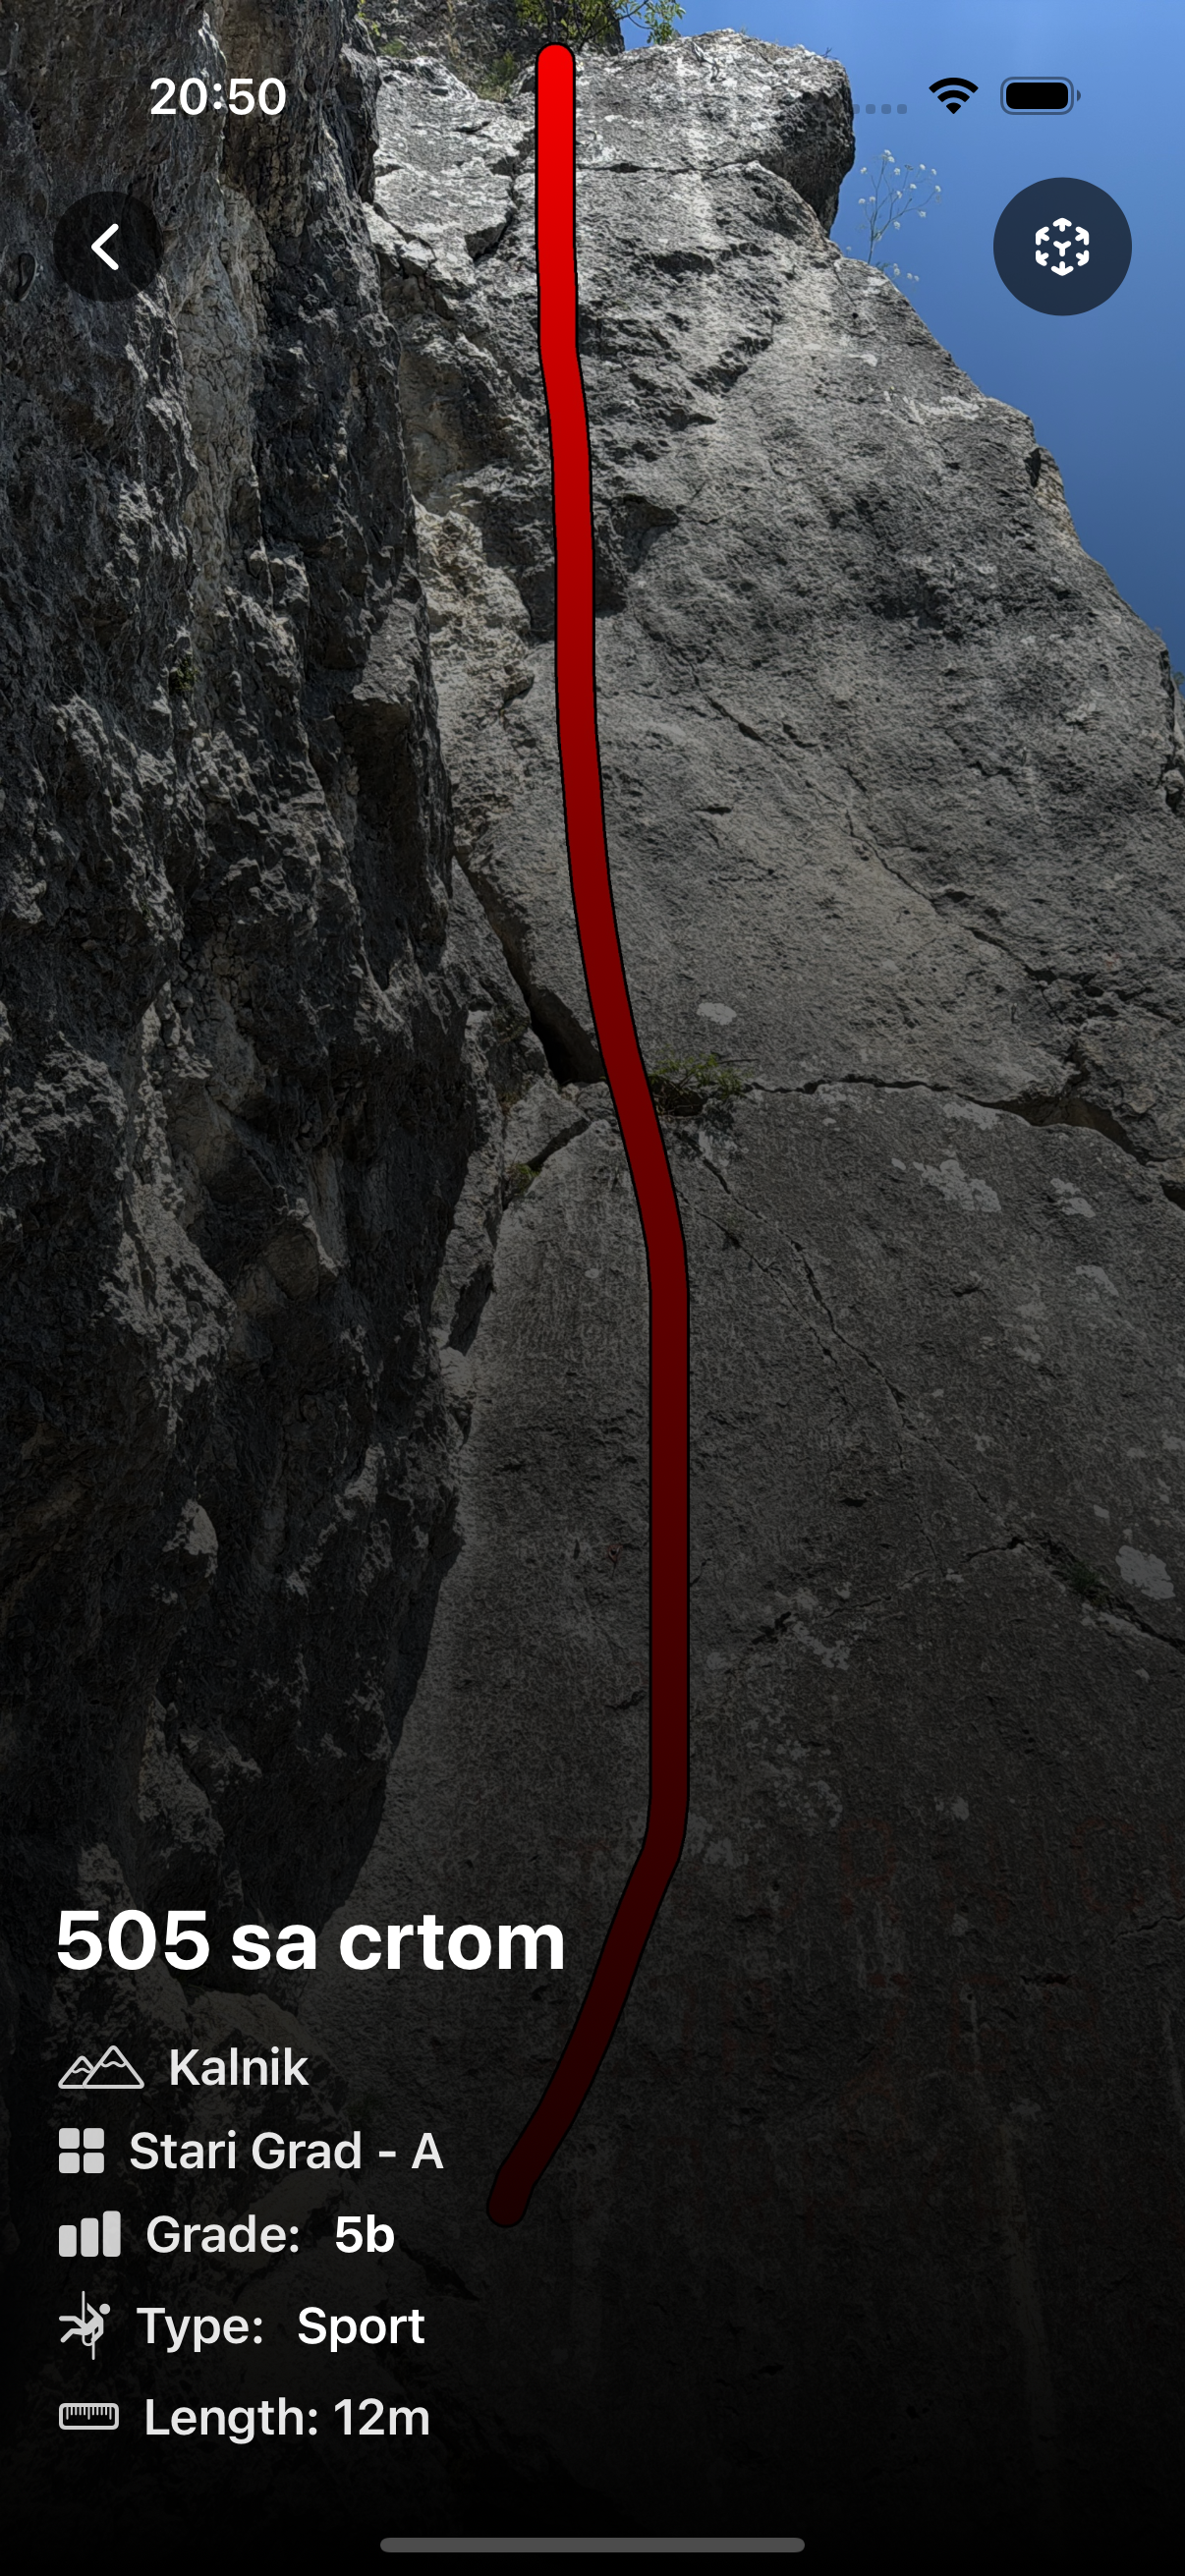
\includegraphics[width=0.8\textwidth]{images/implementacija/offline-mode/offline-route-view.png}
        \caption{Detaljni pregled penjačkog smjera}
        \label{fig:izvanmrezni_nacin_rada_detail_route}
    \end{subfigure}
    \caption{Izvanmrežni način rada - detaljni pregledi penjališta i penjačkog smjera}
    \label{fig:izvanmrezni_nacin_rada_detail}
\end{figure}

Detaljni pregled penjališta (slika~\ref{fig:izvanmrezni_nacin_rada_detail_crag}) i smjerova (slika~\ref{fig:izvanmrezni_nacin_rada_detail_route}) zadržava sve ključne informacije i komponente, s iznimkom onih koje ovise o vanjskim servisima, poput vremenske prognoze i uređivanje podataka.
Najvažnije, funkcionalnost prepoznavanja penjačkih smjerova pomoću proširene stvarnosti je dostupna u izvanmrežnom načinu rada. Budući da su sve referentne slike pohranjene lokalno, proces detekcije i vizualizacije može se izvršavati neovisno o internetskoj vezi. Time se osigurava da ta funkcionalnost je dostupna penjačima upravo gdje je najpotrebnija - ispred same stijene.
